\documentclass[11pt,a4paper]{article}
\usepackage[utf8]{inputenc}
\usepackage[T1]{fontenc}
\usepackage[portuguese]{babel}
\usepackage{graphicx}
\usepackage{amsmath}
\usepackage{booktabs}
\usepackage{geometry}
\usepackage{listings}
\usepackage{float}
\usepackage{xcolor}

\geometry{margin=2.5cm}
\title{EA/ECAC 2025 --- TP1\\Classificação de Atividades Humanas}
\author{Bernardo Direito --- 2023215454\\Teodoro Marques --- 2023211717}
\date{\today}

\lstset{
    language=Python,
    basicstyle=\footnotesize\ttfamily,
    keywordstyle=\color{blue},
    stringstyle=\color{red},
    commentstyle=\color{green!40!black},
    breaklines=true,
    showstringspaces=false,
    upquote=true
}

\begin{document}
\maketitle

\section{Introdução}
O presente relatório detalha a implementação de uma pipeline de análise de dados para o reconhecimento de atividades humanas (Human Activity Recognition - HAR), utilizando o dataset FORTH-TRACE. O objetivo principal é exercitar os conceitos fundamentais de uma pipeline de análise de dados, desde a preparação e limpeza dos dados até à extração, seleção e redução de características.

O trabalho está estruturado de acordo com as tarefas propostas no guião do Trabalho Prático 1 (TP1.pdf). Cada secção deste relatório corresponde a uma tarefa, explicando a metodologia adotada, as funções implementadas no script \texttt{mainActivity.py}, e os resultados obtidos, incluindo gráficos e tabelas.

\section{Tarefa 2: Carregamento de Dados}
A primeira etapa consistiu em desenvolver uma função para carregar os dados de um participante a partir dos ficheiros CSV. A função \texttt{carregar_dados_participante} lê os 5 ficheiros de um determinado participante e concatena-os num único array NumPy para facilitar a manipulação posterior.

\begin{lstlisting}[caption={Função para carregar os dados de um participante.}, label={lst:load_data}]
def carregar_dados_participante(num_participante, base_dir="."):
    """
    (Tarefa 2) Le todos os 5 ficheiros CSV do participante e devolve um array NumPy.
    """
    part_dir = os.path.join(base_dir, f"part{num_participante}")
    dados = []

    for i in range(1, 6): # Dispositivos 1 a 5
        caminho_ficheiro = os.path.join(part_dir, f"part{num_participante}dev{i}.csv")
        try:
            with open(caminho_ficheiro, newline='') as csvfile:
                leitor = csv.reader(csvfile)
                for linha in leitor:
                    try:
                        dados.append([float(x) for x in linha])
                    except ValueError:
                        continue
        except FileNotFoundError:
            print(f"[Aviso] Ficheiro nao encontrado: {caminho_ficheiro}")
        except Exception as e:
            print(f"[Erro] Problema ao ler {caminho_ficheiro}: {e}")

    if not dados:
        return np.array([])
        
    return np.array(dados)
\end{lstlisting}

\section{Tarefa 3: Análise e Tratamento de Outliers}

Nesta tarefa, o objetivo foi identificar e tratar outliers utilizando diferentes abordagens, univariadas e multivariadas.

\subsection{3.1: Boxplot de Atividades}
Para visualizar a distribuição dos dados e a presença de outliers, foram gerados boxplots para cada uma das 16 atividades. Estes gráficos foram criados para os módulos dos vetores de aceleração, giroscópio e magnetómetro, separadamente para cada um dos 5 dispositivos.

\begin{figure}[H]
    \centering
    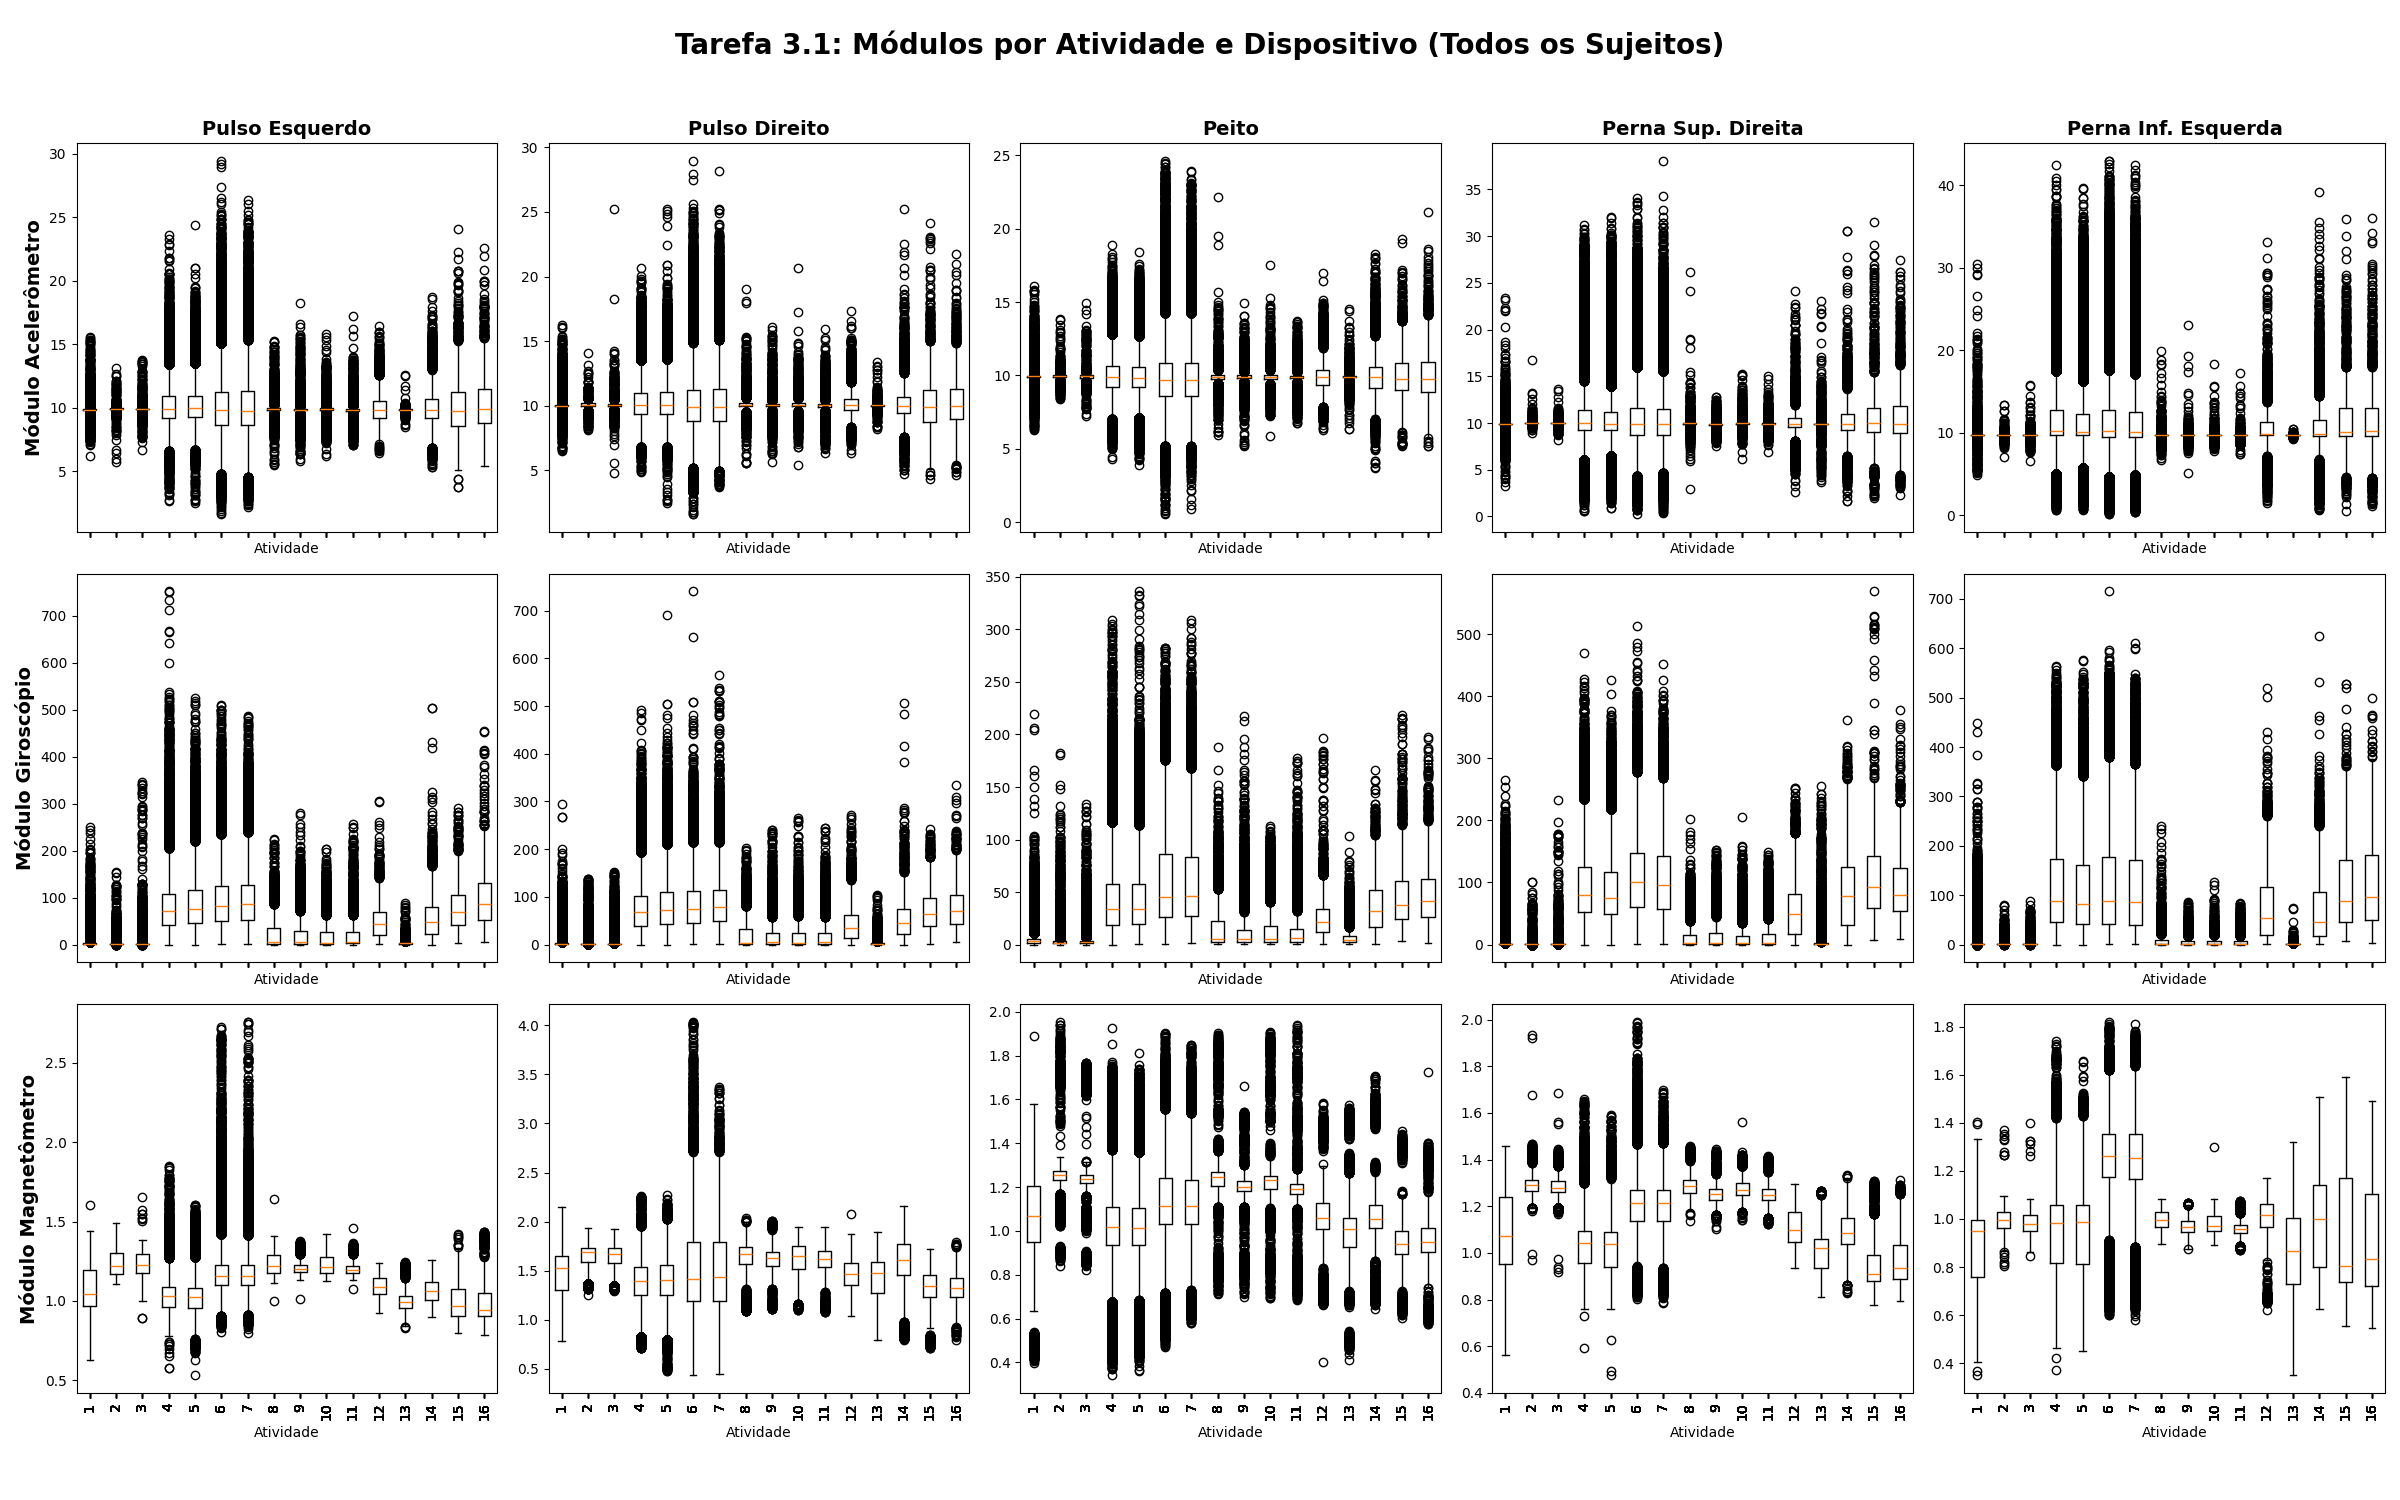
\includegraphics[width=\textwidth]{graphs/meta1_tarefa_3_1_boxplots.png}
    \caption{Tarefa 3.1: Boxplots dos módulos por atividade e dispositivo.}
    \label{fig:boxplots}
\end{figure}

\subsection{3.2: Análise da Densidade de Outliers (IQR)}
Utilizando o método de IQR (Interquartile Range), o mesmo utilizado pelos boxplots, foi calculada a densidade de outliers para o sensor do pulso direito. A tabela abaixo resume os resultados.

\begin{verbatim}
--- Início Tarefa 3.2: Densidade de Outliers (IQR - Pulso Direito) ---
Analisando Sensor: Pulso Direito

| Variável              | Atividade | n_total (nr) | n_outliers (no) | Densidade (d) |
|-----------------------|-----------|--------------|-----------------|---------------|
| Módulo Acelerômetro   |         1 |       157882 |            6624 |          4.20% |
| Módulo Acelerômetro   |         2 |        83968 |             181 |          0.22% |
...
| Módulo Magnetômetro   |        16 |         1905 |              30 |          1.57% |

--- Fim Tarefa 3.2 ---
\end{verbatim}

\subsection{3.3: Rotina Z-Score}
Foi implementada uma função para identificar outliers com base no Z-Score, que mede o desvio de um ponto de dados em termos de desvios padrão da média.

\begin{lstlisting}[caption={Função para identificar outliers com Z-Score.}, label={lst:zscore}]
def identificar_outliers_zscore_3_3(amostras, k):
    if amostras.size == 0:
        return np.array([], dtype=bool)
    media = np.mean(amostras)
    std = np.std(amostras)
    if std == 0:
        return np.zeros(amostras.shape, dtype=bool)
    z_scores = (amostras - media) / std
    return np.abs(z_scores) > k
\end{lstlisting}

\subsection{3.4: Plots Z-Score}
Utilizando a função de Z-Score, foram gerados gráficos de dispersão para visualizar os outliers (a vermelho) e inliers (a azul) para diferentes valores de \(k\).

\begin{figure}[H]
    \centering
    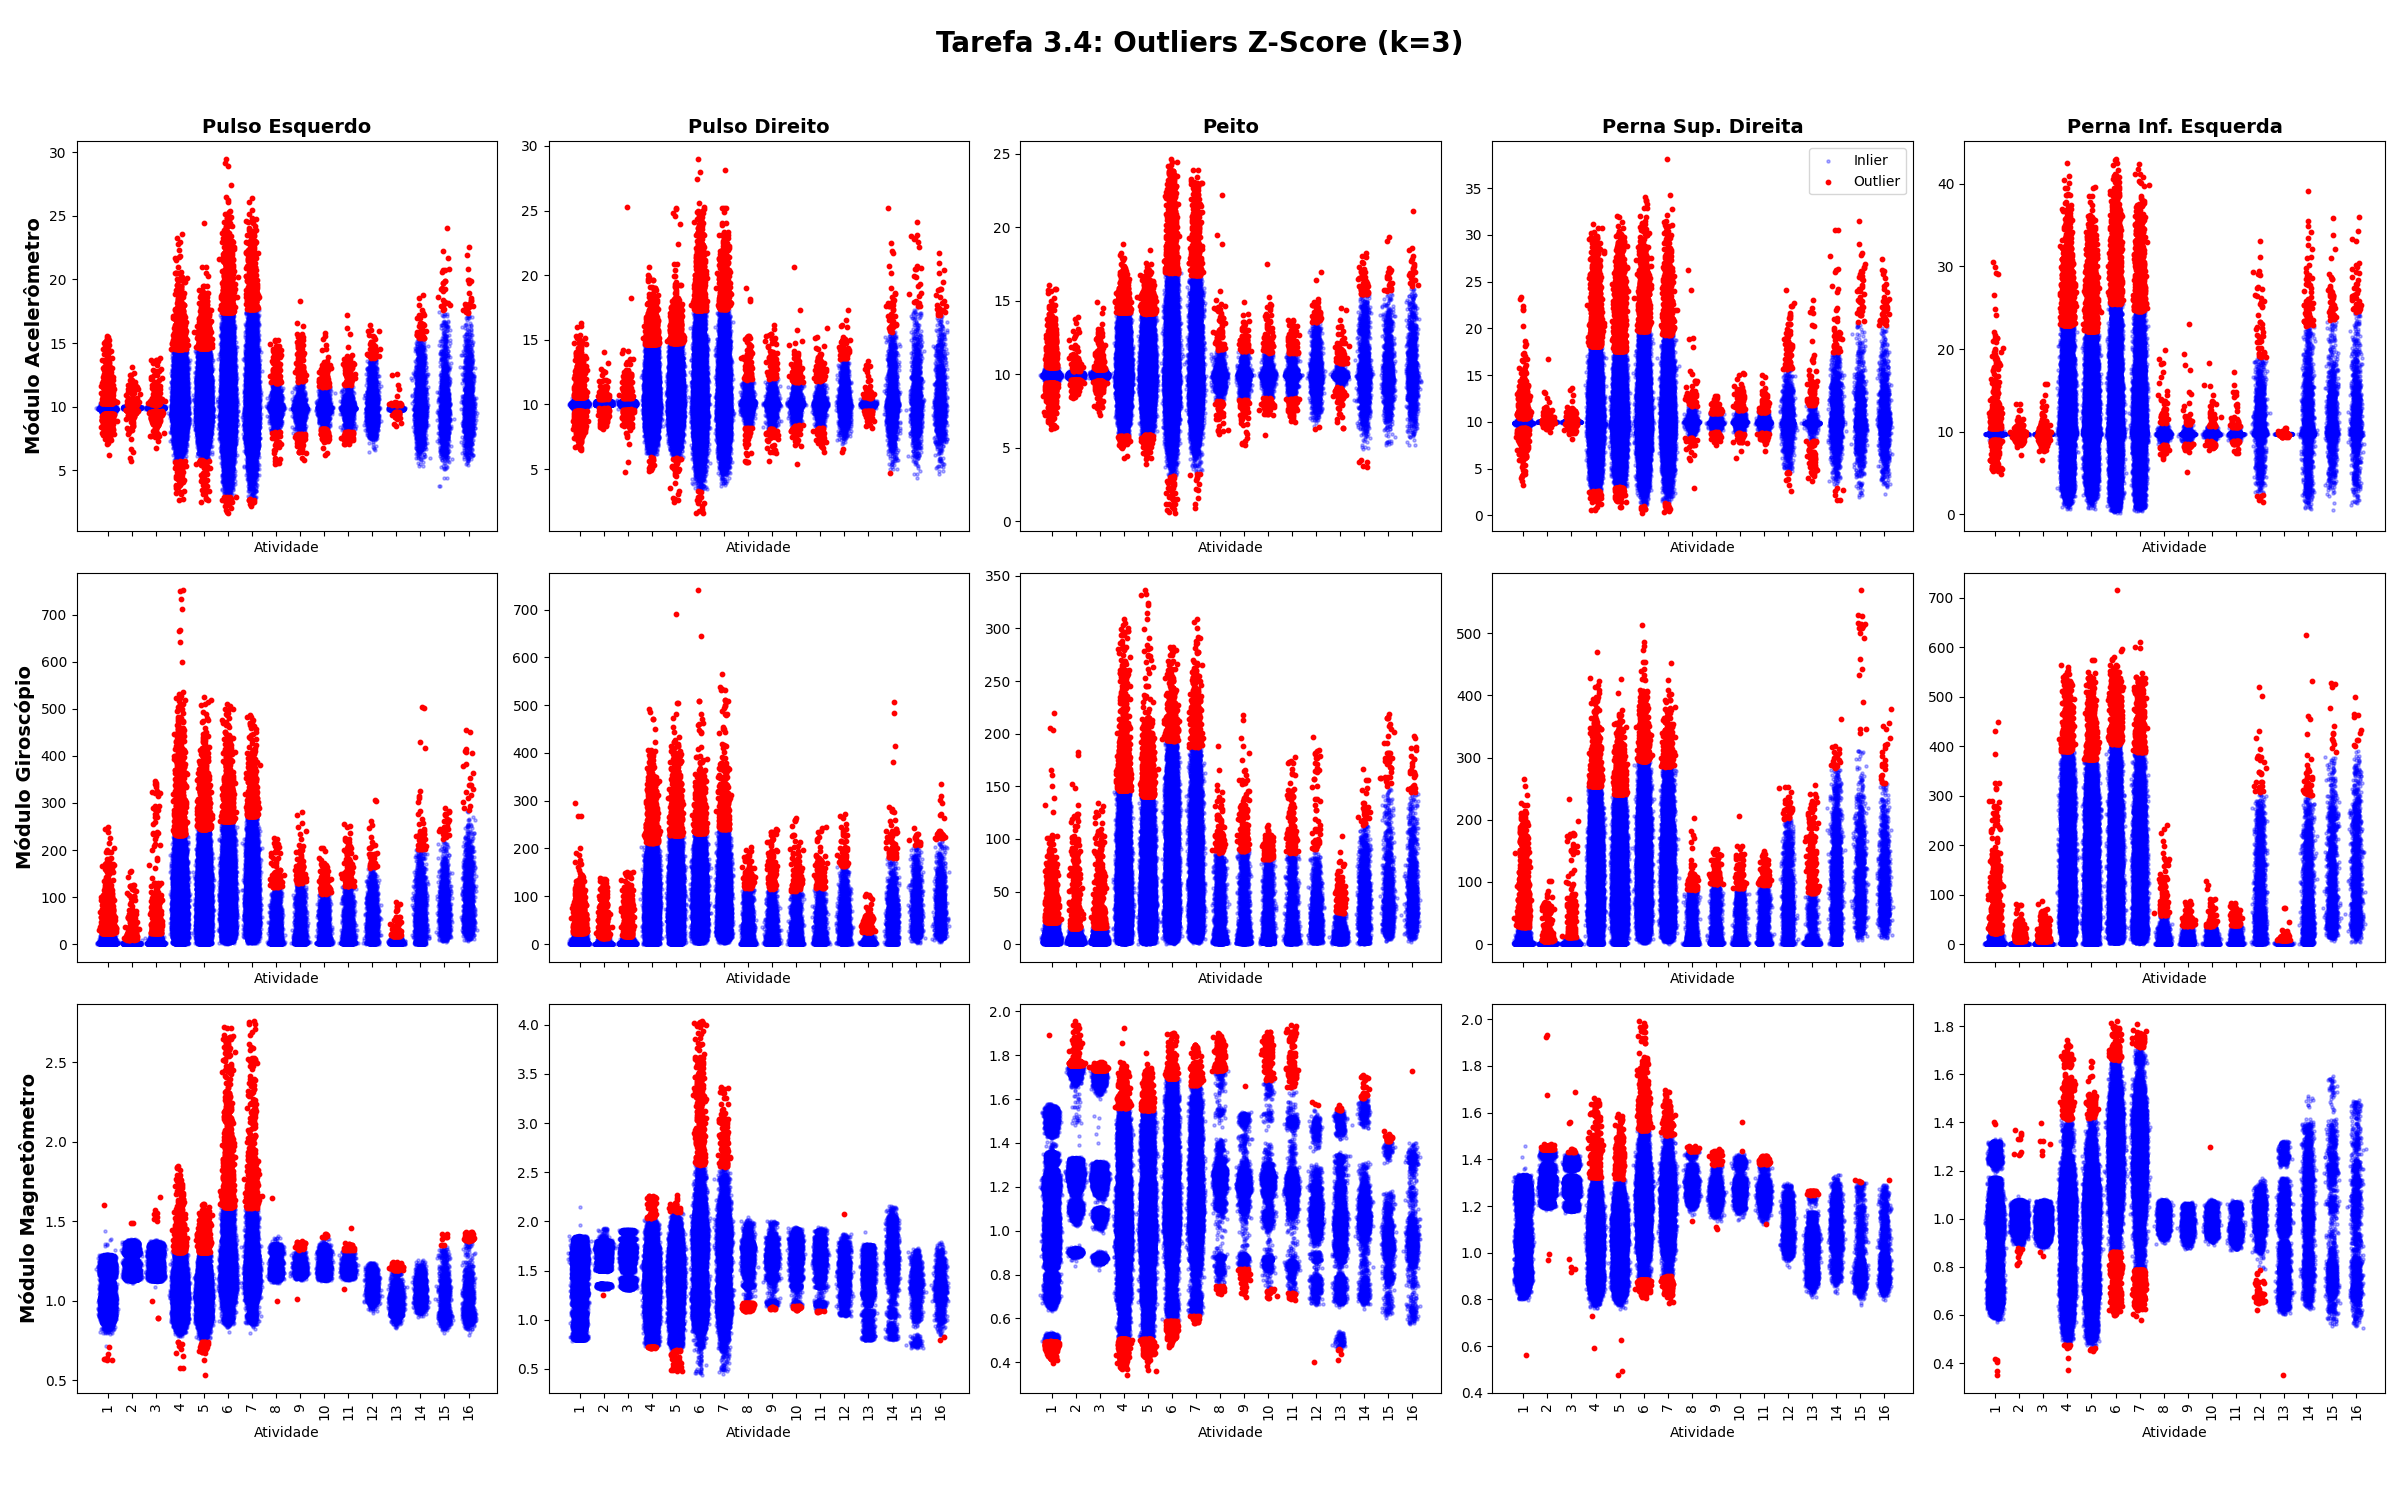
\includegraphics[width=\textwidth]{graphs/meta1_tarefa_3_4_zscore_k3.png}
    \caption{Tarefa 3.4: Outliers identificados com Z-Score para k=3.}
    \label{fig:zscore_plot}
\end{figure}

\subsection{3.5: Comparação IQR vs Z-Score}
Foi gerada uma tabela comparativa das densidades de outliers encontradas pelos métodos IQR e Z-Score (com k=3, 3.5 e 4) para o sensor do pulso direito. A discussão apresentada no output do terminal explica as diferenças, vantagens e desvantagens de cada método.

\subsection{3.6: Rotina K-Means}
Foi implementado o algoritmo K-Means a partir do zero, para agrupar os dados em \(n\) clusters.

\begin{lstlisting}[caption={Implementação do algoritmo K-Means.}, label={lst:kmeans}]
def kmeans_3_6(X, n_clusters, max_iter=100, tol=1e-4, random_state=42):
    rng = np.random.default_rng(random_state)
    indices = rng.choice(X.shape[0], n_clusters, replace=False)
    centroides = X[indices]
    
    for _ in range(max_iter):
        distancias = np.sqrt(((X[:, np.newaxis] - centroides) ** 2).sum(axis=2))
        labels = np.argmin(distancias, axis=1)
        novos_centroides = np.array([X[labels == i].mean(axis=0) for i in range(n_clusters)])
        
        if np.all(np.linalg.norm(novos_centroides - centroides, axis=1) < tol):
            break
            
        centroides = novos_centroides
        
    return centroides, labels
\end{lstlisting}

\subsection{3.7: Outliers com K-Means e Plot 3D}
O K-Means foi utilizado como uma abordagem multivariada para deteção de outliers. Os outliers foram definidos como os pontos mais distantes dos centroides dos seus respetivos clusters. Os resultados foram visualizados em gráficos 3D.

\begin{figure}[H]
    \centering
    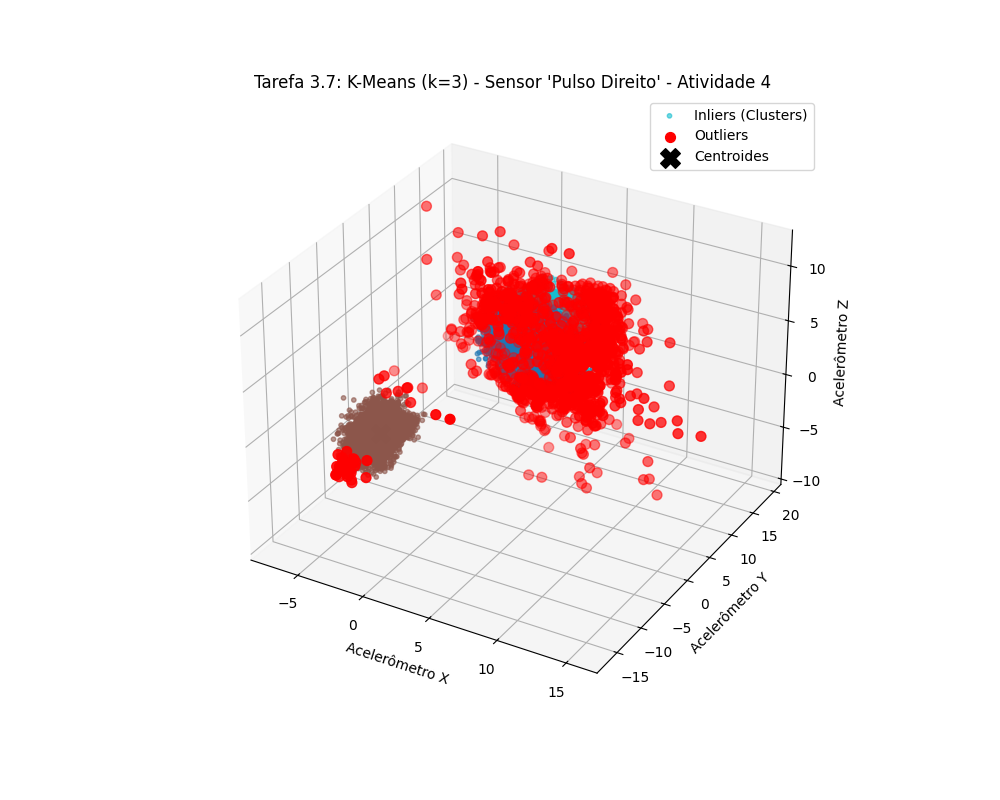
\includegraphics[width=0.7\textwidth]{graphs/meta1_tarefa_3_7_kmeans_k3.png}
    \caption{Tarefa 3.7: Outliers identificados com K-Means (k=3).}
    \label{fig:kmeans_outliers}
\end{figure}

\subsection{3.7.1 (Bónus): Outliers com DBSCAN}
Como bónus, foi utilizado o algoritmo DBSCAN para identificar outliers, que são considerados os pontos de ruído (label -1) pelo algoritmo.

\begin{figure}[H]
    \centering
    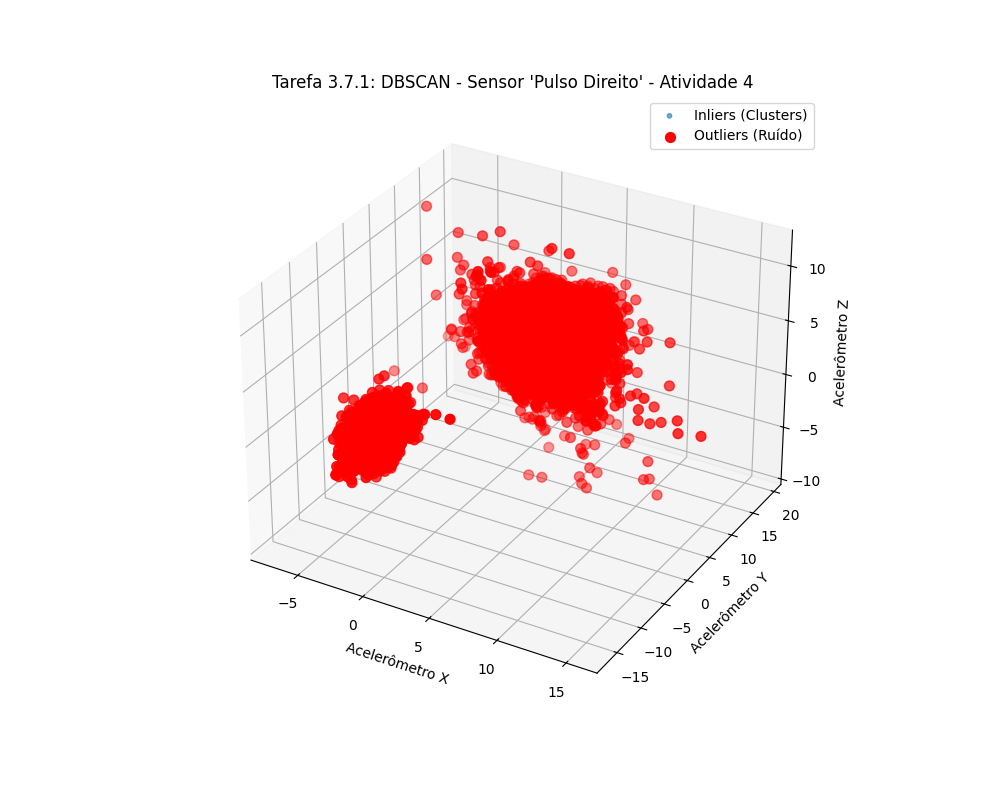
\includegraphics[width=0.7\textwidth]{graphs/meta1_tarefa_3_7_1_dbscan.png}
    \caption{Tarefa 3.7.1: Outliers (ruído) identificados com DBSCAN.}
    \label{fig:dbscan_outliers}
\end{figure}

\section{Tarefa 4: Extração de Informação Característica}

\subsection{4.1: Testes de Significância}
Foram realizados testes estatísticos para determinar se as médias dos módulos das variáveis transformadas são significativamente diferentes entre as várias atividades.

\subsection{4.2: Janelamento e Extração de Features}
Os dados foram segmentados em janelas de 5 segundos com 50% de sobreposição. Para cada janela, foi extraído um vetor de características temporais e espectrais.

\subsection{4.3 e 4.4: PCA}
A Análise de Componentes Principais (PCA) foi aplicada ao conjunto de features para reduzir a sua dimensionalidade. O número de componentes foi escolhido para explicar 75% da variância total.

\begin{figure}[H]
    \centering
    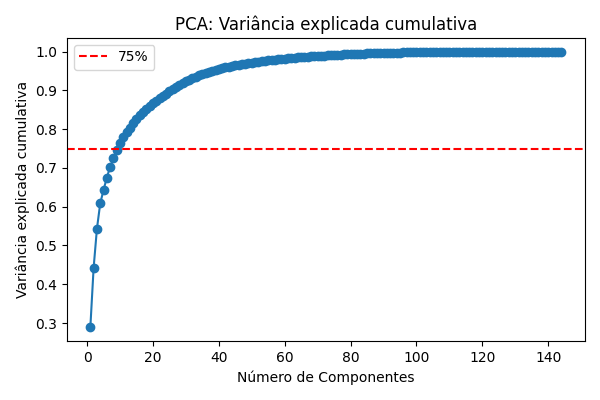
\includegraphics[width=0.6\textwidth]{graphs/tarefa4_pca_variancia.png}
    \caption{Tarefa 4.4: Variância explicada cumulativa pelo PCA.}
    \label{fig:pca}
\end{figure}

\subsection{4.5 e 4.6: Fisher Score e ReliefF}
Foram implementados os métodos de seleção de features Fisher Score e ReliefF para classificar as features mais discriminativas. As 10 melhores features de cada método foram apresentadas.

\begin{verbatim}
Top-10 features (Fisher):
   1. dev1_gyr_mod_spec_entropy  (score=6.7671e+13)
   2. dev1_acc_z_spec_centroid  (score=6.5599e+13)
   ...
Top-10 features (ReliefF):
   1. dev1_gyr_y_spec_dom_freq  (score=-0.6515)
   2. dev1_gyr_z_spec_dom_freq  (score=-0.6415)
   ...
\end{verbatim}

\section{Conclusão}
Este trabalho prático permitiu a aplicação de uma pipeline completa de análise de dados a um problema de reconhecimento de atividades humanas. Foram exploradas várias técnicas para tratamento de outliers, extração e seleção de features.

Os resultados demonstram a importância de cada etapa da pipeline. A análise de outliers revelou diferentes densidades dependendo do método utilizado. A extração de features gerou um espaço de características rico, e a seleção de features com PCA, Fisher Score e ReliefF permitiu identificar as características mais relevantes para a discriminação das atividades.

Como trabalho futuro, sugere-se a utilização das features selecionadas para treinar e avaliar diferentes modelos de classificação, completando assim o ciclo da pipeline de HAR.

\end{document}